% 2023.02.14: lecture 01
\documentclass[../main.tex]{subfiles}
\begin{document}

\section{Деревья разбиения}

\subsection{Граф $G^{\S}$ и его свойства.}

Пусть $G$ - связный граф, тогда:

\begin{df*}[Точка сочленения]
	Вершина $a \in V(G)$ называется \textbf{точкой сочлененияы}, если граф  $G - a$ несвязен.
\end{df*}

\begin{df*}[Блок]
	\textbf{Блоком} называется любой максимальный по включению подграф графа $G$, не содержащий точек сочленения.
\end{df*}

\begin{df*}[Дерево блоков и точек сочленения]
	\textbf{Дерево блоков и точек сочленения} $B(G)$ это двудольный граф, вершины одной доли которого соответствуют всем точкам сочленения  $a_1, \ldots, a_n$ графа $G$, а вершины второй доли соответствуют блокам  $B_1, \ldots, B_m$.

	Вершины  $a_i$ и  $B_j$ соединены ребром  $\iff a_i \in B_j$.
\end{df*}

\begin{df*}[Дерево разбиения] \label{definition:tree_of_partition}
	Пусть $G$ - $k$-связный граф, $\S \subset \R_k(G)$, причем все множества набора $\S$ попарно независимы.

	Тогда \textbf{деревом разбиения} $T(G, \S)$ называется двудольный граф, вершины одной доли это множества из $\S$, а другой части $\Part(\S)$.

	Вершины $S \in \S$ и $A \in \Part(\S)$ смежны $\iff S \subset A$.
\end{df*}

\begin{df*}[$G^{\S}$]
	Пусть $G$ - $k$-связный граф, $\S \subset \R_k(G)$, причем все множества набора $\S$ попарно независимы.

	Тогда граф $G^\S$ это граф $G$ в котором каждое $S \in \S$ дополнили до клики, т.е. провели все пары ребер, которые не присутствовали в $G$.
\end{df*}

\begin{customlm}{1.1} \label{lemma:1_1}
	Выполняется: $\S \subset \R_k(G^\S)$.

	Более того, $\Part(G; \S) = \Part(G^\S, \S)$.
\end{customlm}

\begin{proof}
	Понятно, что если две вершины разделены в $G^\S$, то они разделены и в $G$.

	В обратную сторону, если вышло так что вершины $a, b$ отделены каким то множеством $S \in \S$ в  $G$, а в  $G^\S$ все равно существует путь после удаления $S$, то тогда можно сказать что этот путь проходит в какой то момент по ребру  $(c,d) \in E(G^\S) \setminus E(G)$ и при этом не существует пути $cd$ по ребрам $E(G)$(ведь тогда это ребро на пути можно заменить целиком путем из $E(G)$).

	А значит, что вершины $c, d$ лежат в каком то другом множестве из  $\S$ и при этом их отделяет множество  $S$, противоречие с попарной независимостью множеств~$\S$.
\end{proof}

\begin{customlm}{1.2} \label{lemma:1_2}
	Пусть $G$ - $k$-связный граф, $\S \subset \R_k(G)$ и все множества $\S$ попарно независимы.

	Тогда для произвольного $\T \subset \S, B \in \Part(G; \T)$ и $R \in \R(G^\S(B))$ такого что, $R$ не содержит рёбра, соединяющие пары вершин, входящих в какое-либо множество набора $\S$.
	
	Тогда $R \in \R(G)$.

	В частности, граф  $G^\S(B)$ является $k$-связным.
\end{customlm}

\begin{proof}

	Предположим, что $R \not \in \R(G)$.

	Пусть $x, y \in B$ и множество  $R$ отделяет $x$ и $y$ в $G^\S(B)$, но не отделяет в $G$.
	Тогда по Лемме \ref{lemma:1_1} $R$ не отделяет $x$ и $y$ и в $G^\S$.

	Тогда рассмотрим кратчайший путь  $xy$ в $G^\S - R$, назовем этот путь $P$.

	Предположим что путь $P$ содержит $z \not \in B$, но тогда существует $T \in \T$, которое отделяет $z$ от $B$.
	Тогда двигаясь по пути $P$ мы как минимум дважды войдем в $T$, обозначим эти вершины $a, b$.

	По условию $ab \not \in R$, а следовательно в $G^\S$ есть ребро $(a,b)$.
	Значит можно выкинуть кусок пути и укоротить путь.
	Рисунок \ref{fig:lemma_1_2}.

\begin{figure}[ht]
    \centering
	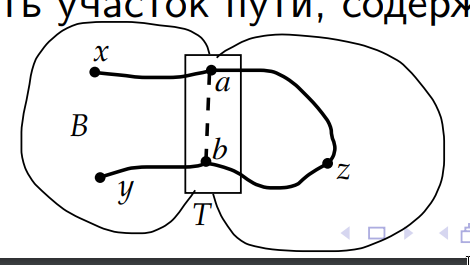
\includegraphics[width=0.3\columnwidth]{figures/lemma_1_2.png}
    \caption{Рисунок к лемме \ref{lemma:1_2}}
    \label{fig:lemma_1_2}
\end{figure}

	Отсюда следует что $P \subset B$, значит $P$ путь в  $G^\S(B) - R$, но такого пути нет ведь $R$ разделяет $x$ и $y$.
	Следовательно, $R$ разделяет  $x$ и  $y$ в $G$, а значит $R \in \R(G)$.

	В завершении добавим, что $\R_{k-1}(G) = \varnothing$, а значит и  $\R_{k - 1}(G^\S(B)) = \varnothing$, следовательно $G^\S(B)$ - $k$-связный.
	
\end{proof}

\subsection{Дерево разбиения $k$-связного графа набором из попарно независимых k-разделяющих множеств.}

\begin{customthm}{1.1} \label{theorem:1_1}
	Пусть $G$ -  $k$-связный граф, $\S \subset \R_k(G)$ - набор попарно независимых множеств.
	Тогда выполняются следующие утверждения:

	 \begin{enumerate}
		 \item $\wT(G, \S)$ - это дерево \label{stmt:theorem_1_1_1}
		 \item Для каждого множества $S \in \S$ выполняется  $\deg_{\wT(G, \S)}(S) = |\Part(S)|$.
			 Более того, для каждой части  $A \in \Part(S)$ существует единственная часть  $B \in \Part(\S) \colon B \subset A$ и  $B$ смежна с  $S$ в  $\wT(G, \S)$ \label{stmt:theorem_1_1_2}
		 \item Все висячие вершины дерева  $\wT(G, \S)$ соответствуют частям  $\Part(\S)$ \label{stmt:theorem_1_1_3}
		 \item Множество  $S$ разделяет части  $B, B' \in \Part(\S)$ в графе  $G \iff$ когда  $S$ разделяет  $B, B'$ в  $T(G, \S)$ \label{stmt:theorem_1_1_4}
	\end{enumerate}
	
\end{customthm}

\begin{proof}
	Заметим, что Утверждение \eqref{stmt:theorem_1_1_3} следует из Утверждения \eqref{stmt:theorem_1_1_2}, потому что $|\Part(S)| \geqslant 2$.

	Рассмотрим  $G^* = G^\S$.
	По Лемме \ref{lemma:1_1} следует, что разбиения графов  $G$ и  $G^*$ набором  $\S$ совпадают. Обозначим это разбиение за  $\Part(\S)$.

	Тогда  $T(G, \S) = T(G^*, \S)$, поэтому докажем утверждения теоремы для графа  $G^*$.

	Пусть $S \in \S, \Part(S) = \{A_1, \ldots, A_n\}, G_i = G^*(A_i)$.
	По Лемме \ref{lemma:1_2} все графы $G_1, \ldots, G_n$ являются  $k$-связными.

	Пусть набор  $\S_i$ состоит из всех множеств набора  $\S$, лежащих в  $A_i$ и отличных от  $S$.

	Тогда каждое множество из  $\S \setminus \{S\}$ лежит ровно в одном из наборов $\S_1, \ldots, \S_n$, по Лемме \ref{lemma:0_4}.

	Для каждого $i$ пусть $U_i \in \Part(G_i;\S_i)$ - часть, содержащая  $S$.
	По Лемме \ref{lemma:1_2}, для любой части $U \in \Part(G_i;\S_i)$ граф $G^*(U)$ является  $k$-связным, а значит, его не разделяет ни одно из множеств набора  $\S$, не лежащих в  $U$. 

	Множество $S$ лежит в части  $U_i$, но также не разделяет ее, т.к. $U_i \subset A_i \in \Part(G;S)$.
	Это означает, что  $\Part(G_i;\S_i) \subset \Part(G^*; \S)$, причем именно  $U_i$ содержит  $S$.

	Следовательно, $\Part(G^*; \S) = \bigsqcup\limits_{i=1}^n \Part(G_i;\S_i)$, а части  $\Part(\S)$, содержащие множество  $S$ - это  $U_1, \ldots, U_n$.
	Таким образом Утверждения \eqref{stmt:theorem_1_1_2} и \eqref{stmt:theorem_1_1_4} доказаны для множества  $S$, для остальных множеств из  $\S$ доказательство аналогично.

\begin{figure}[ht]
    \centering
	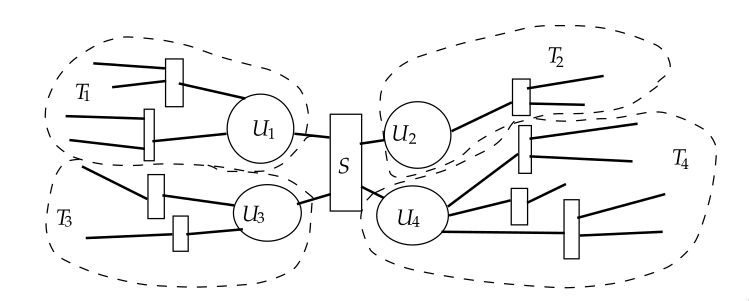
\includegraphics[width=0.5\columnwidth]{figures/theorem_1_1.png}
    \caption{Рисунок к Теореме \ref{theorem:1_1}}
    \label{fig:theorem_1_1}
\end{figure}

	Чтобы показать Утверждение \eqref{stmt:theorem_1_1_1}, воспользуемся индукцией по количеству элементов в наборе $\S$ и при это не фиксируем  $k, G$.
	Теперь скажем что каждая часть $\Part(G_i; \S_i)$, кроме  $U_i$ смежна в  $T_i = T(G_i, \S_i)$ с теми же вершинами, что в  $T(G, \S)$.
	Для части  $U_i$ в  $T(G, \S)$ добавляется ребро к множеству  $S$.

	Поэтому  $T(G, \S) - S$ распадается ровно на  $n$ связных подграфов: это графы  $T_i$, где  $i \in [n]$.
	По индукционному предположению, все эти графы - деревья.

\end{proof}

\subsection{Дерево разбиения $k$-связного графа множеством попарно независимых разрезов — две конструкции и их свойства.}

\begin{df*}[Дерево разрезов]
	Пусть $G$ ~--  $k$-связный граф, $\S \subset \T(G)$ ~-- множество попарно независимых разрезов, причем в $\S$ нет двух разрезов, содержащих одно и то же ребро.

	Тогда \textbf{деревом разрезов} множества $\S$ назовем двудольный граф $\BT(G, \S)$, в одной доли будут разрезы  $\S$, а во второй части  $\Part(\S)$, причем $S \in \S$ и часть  $A \in \Part(\S)$ смежны $\iff A$ содержит одну из границ разреза $S$. 
\end{df*}

\begin{df*}[Крайная часть]
	Если часть $A \in \Part(\S)$ соответствует висячей вершине дерева  $\BT(G, \S)$, то назовем такую часть \textbf{крайней}.
\end{df*}

\begin{customthm}{1.2} \label{theorem:1_2}
	Верны следующие утверждения:

	\begin{enumerate}
		\item $\BT(G, \S)$ ~-- дерево 
		\item Любой разрез  $S \in \S$ смежен в  $\BT(G, \S)$ ровно с двумя частями  $\Part(\S)$, причем эти две части содержатся в разных частях  $\Part(S)$
		\item Разрез  $S \in \S$ отделяет вершину  $B$ от вершины  $C$ в  $\BT(G, \S) \iff S$ отделяет  $B$ от  $C$ в графе  $G$
		\item Если крайняя часть  $A \in \Part(\S)$ смежна в  $\BT(G, \S)$ с разрезом  $T$, то  $A \in \Part(T)$
		\item Крайние части  $\Part(\S)$ это в точности минимальные по включению части разбиения графа  $G$ одним разрезом из множества  $\S$.
	\end{enumerate}

\end{customthm}

\begin{proof}
	Индукция по количеству разрезов в $\S$.
	База  $|\S| = 1$ очевидна.

	Пусть для любого меньшего  $\S$ множества разрезов утверждение верно, тогда:

	Выберем разрез $T \in \S$ так, что одна из частей  $B \in \Part(T)$ ~-- минимальная по включению среди всех частей разбиения графа  $G$ одним разрезом из $\S$.

	Пусть $\S' = \S \setminus \{T\}$. Тогда граф $\BT(G, \S')$ ~-- дерево.

	Пусть  $\Part(T) = \{B, B'\}$.
	Рассмотрим разрез  $S \in \S'$, т.к.  $S$ и  $T$ независимы и в силу минимальности  $B \in \Part(T)$ существует часть  $A_S \in \Part(S) \colon B \subset A_S$, пусть $\Part(S) = \{A_S, A_S'\}$, тогда  $B' \supset A_S'$.

	По Лемме \ref{lemma:0_8} имеем  $A_S' \not \supset R(B)$.

	Рассмотрим квазичасть $A = \bigcap_{S \in \S'} A_S \quad \in \QPart(\S')$.

	Любая отличная от  $A$ часть  $A' \in \Part(\S')$ лежит в $A_S'$ для некоторого $S \in \S'$ и поэтому $A' \not \supset R(B)$.

	По Теореме \ref{theorem:0_3} части $D \in \Part(\S)$ ~-- это максимальные по включению множества вида:

	\begin{align} \label{eq:1_thm_2}
		D = H \cap F, \quad \text{ где } H \in \Part(T) \text{ и } F = \bigcap_{S \in \S'} F_S \in \Part(\S')
	\end{align}

	Разберем несколько случаев:

	\begin{itemize}
		\item $F \neq A$.
			Тогда для некоторого $S \in S'$ имеем $F_S \neq A_S$ и поэтому $F_S = A_S'$, следовательно $B' \supset A_S' = F_S \supset F$.
			Поэтому  $B \cap F \subsetneq F = B' \cap F$.

			Следовательно, все максимальные по включению множества вида \eqref{eq:1_thm_2}, где  $F \neq A$ ~-- это части $F \in \Part(\S')$ и только они.

\begin{figure}[ht]
    \centering
	\incfig[0.4]{theorem_1_2}
	\caption{Рисунок к Теореме \ref{theorem:1_2}.}
    \label{fig:theorem_1_2}
\end{figure}

			Таким образом, части $\Part(\S') \setminus \{A\} \subset \Part(\S)$.

			Заметим, что по Лемме \ref{lemma:0_8} часть $F_S = A'_S$ не содержит ни одно из множеств $R(B)$ и $R(B')$, следовательно, $F$ не смежна в $\BT(G, \S)$ с разрезом $T$. Таким образом, $\N_{\BT(G, \S)}(F) = N_{\BT(G, \S')}(F)$.

		\item $F = A, H = B \implies D = B \cap A$.

			$D = A \cap B = B$, понятно, что $B$ ~-- максимальное по включению множество вида \eqref{eq:1_thm_2}, а значит $B \in \Part(\S)$.

			По Лемме \ref{lemma:0_8} часть $B$ не содержит никаких границ разрезов множества $\S'$, следовательно, $B$ ~-- висячая вершина дерева $\BT(G, \S)$, смежная только с разрезом $T$.

		\item $F = A, H = B' \implies D = B' \cap A$.

			По Лемме \ref{lemma:0_8} часть $B' $ содержит все границы разрезов из $\S'$, которые лежат в $A$.

			И по Лемме \ref{lemma:0_8} для всех $S \in S'$ имеем $A_S \supset R(B')$, а значит $A \supset R(B')$.

			Тогда $D$ содержит $R(B')$ и все границы разрезов из $S'$, лежащие в $A$, а других границ разрезов из $\S$ не содержит. Это означает, что $\N_{\BT(G, \S)}(D) = \N_{\BT(G, \S')}(A) \cup \{T\}$.

			Таким образом, граф $\BT(G, \S)$ получается из $\BT(G, \S')$ переименованием вершины $A$ в $D$, присоединением к $D$ разреза $T$, а к $T$ ~-- части $B$.

\begin{figure}[ht]
    \centering
	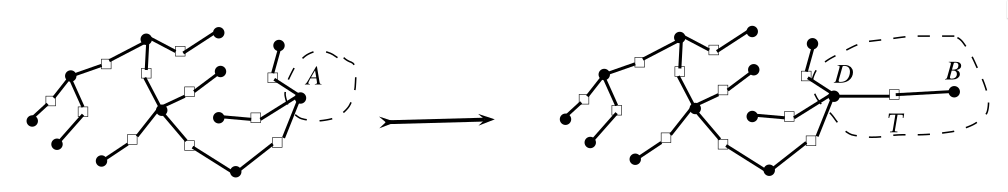
\includegraphics[width=0.6\columnwidth]{figures/theorem_1_2_case_3.png}
	\caption{Рисунок к 3 случаю Теоремы \ref{theorem:1_2}.}
    \label{fig:theorem_1_2_case_3}
\end{figure}

	\end{itemize}

	Из вышесказанного ясно, что $\BT(G, \S)$ ~-- дерево, поэтому 1 утверждение доказано.

	Заметим, что разрез $T$ смежен в этом дереве с двумя частями, содержащими его границы, это $B$ и $D \subset B'$, а других таких частей нет. Поэтому утверждение 2 выполнено.

	Теперь про утверждение 3.

	Мы доказали, что часть $B' \in \Part(T)$ содержит все отличные от $B$ части $\Part(\S)$, а также для каждого разреза $S \in \S$ часть $B'$ содержит часть $A'_S \in \Part(S)$.

	Это означает, что разрез $T$ отделяет крайнюю часть $B$ от всех остальных частей и разрезов как в $\BT(G, \S)$, так и в графе $G$. Более того, $T$ не отделяет друг от друга в графе $G$ никакие отличные от $B$ части $\Part(\S)$ и разрезы из $\S'$, т.к. они все лежат в $B' \in \Part(T)$.

	Теперь рассмотрим любой $S \in \S'$.

	 По индукционному предположению для дерева $\BT(G, \S')$, утверждение верно для разрезов из $S'$ и частей $\Part(\S)$, являющихся частями $\Part(S')$, а по доказанному выше это все части $\Part(S)$, кроме $B$ и $D = A \cap B'$.

	 Разрез $S$ не отделяет в дереве $\BT(G, \S')$ часть $A \in \Part(\S')$ от остальных частей и разрезов, лежащих в $A_S$, отметим что  $A_S \supset A = D \cap B$, тогда по Лемме \ref{lemma:0_8} имеем $A_S \supset W(T)$, теперь из построения $\BT(G, \S)$ следует утверждение 3.

	 Посмотрим на 4 утверждение. Понятно, что оно верно для части $B$.

	 Любая другая крайняя часть соответствует висячей вершине дерева $\BT(G, \S')$, поэтому для нее утверждение верно по индукции.

	 И последнее, 5 утверждение.

	 По индукционному предположению крайние части  $\Part(\S')$ это в точности минимальные по включению среди всех частей разбиения графа $G$ одним разрезом из $\S' $. Рассмотрим такую часть $H$.

	 Если $H \neq A$, то $H \subset B' \in \Part(T)$, поэтому часть $H$ останется минимальной.

	 Остается отметить, что $A \in \Part(\S')$ не является минимальной, ведь $A \supsetneq B$ и не является крайней частью.

\end{proof}

\begin{df*}[$\PT(G, \S)$]
	Построим граф $\PT(G, \S)$ следующим образом: вершины этого графа ~-- части из $\Part(\S)$, причем две части $A, B \in \Part(\S)$ смежны $\iff$ они содержат границы одного и того же разреза $\S$.
\end{df*}

\begin{customcrly}{1.1} \label{crly:1_1}
	Верны следующие утверждения:

	\begin{enumerate}
		\item Граф $\PT(G, \S)$ ~-- дерево 
		\item Каждому ребру $AB$ графа $\PT(G, \S)$ поставим в соответствие разрез из $\S$, границы которого содержатся в частях $A$ и $B$.
			Тогда это отображение взаимно однозначное соответствие между рёбрами $\PT(G, \S)$ и разрезами из $\S$.
		\item $|\Part(\S)| = |\S| + 1$
		\item Пусть  $R$ ~-- граница одного из разрезов $\S$, тогда существует ровно одна часть $\Part(\S)$ содержащая $R$
		\item Если части  $A, B \in \Part(\S)$ смежны в дереве $\BT(G, \S)$ с одним разрезом $S$, то $A \cap B = V(S)$
		\item Если части  $A, B \in \Part(\S)$ смежны в дереве $\PT(G, \S)$, то $|A \cap B| \leqslant k - 1$
	\end{enumerate}
 
\end{customcrly}

\begin{proof}
	По Теореме \ref{theorem:1_2} граф $\BT(G, \S)$ ~-- дерево, причем все его вершины соответствующие разрезам имеют в $\BT(G, \S)$ степень 2.

	Тогда из пункта 2 Теореме \ref{theorem:1_2} понятно, что заменив в этом дереве каждый разрез $S \in \S$ на ребро, соединяющие две смежные с ним в $\BT(G, \S)$ части $\Part(\S)$ мы получим дерево $\PT(G, \S)$, откуда получаем что утверждения 1, 2 верны.

	Пункт 3 следует из пункта 2.

	Пункт 4 следует из пункта 2 Теоремы \ref{theorem:1_2}.

	По Теореме \ref{theorem:1_2} части $A$ и $B$ содержат разные границы разреза $S$, поэтому $A \cap B \supset V(S)$, но разрез  $S$ отделяет $A$ от $B$, а поэтому $V(S) \supset A \cap B $, откуда получаем утверждение 5.

	Части $A$ и $B$ смежны в дереве $\BT(G, \S)$ с одним разрезом $S$, таким образом пункт 6 следует из пункта 5.
\end{proof}

\subsection{Гипердерево и его свойства.}

\begin{df*}[Гипердерево]
	Гиперграф $H$ называется \textbf{гипердеревом}, если он связен, ни одного его гиперребро не является подмножеством другого и для любого цикла в этом гиперграфе существует гиперребро, содержащее все его вершины.
\end{df*}

\begin{df*}[Крайняя вершина]
	Назовем вершину $v$ гипердерева $H$ крайней, если гиперграф $H - v$ связен.
\end{df*}

\begin{df}[$T(H)$]
	По гиперграфу $H$ построим двудольный граф $T(H)$, вершины одной доли которого ~-- вершины $H$, а вершины другой доли ~-- гиперребра $H$.
	Каждое гиперребро $R$ соединим со всеми вершинами которые оно содержит.
\end{df}

\begin{customthm}{1.3} \label{theorem:1_3}
	Пусть $H$ ~-- гипердерево, $|V(H)| \geqslant 2$, тогда выполнены следующие утверждения:

	\begin{enumerate}
		\item Граф $T(H)$ ~-- дерево
		\item Никакие два гиперребра $H$ не имеют двух общих вершин
		\item Пусть $a \in V(H)$. Тогда $\deg_H(a)$ равняется кол-ву компонент связности гиперграфа $H - a$. Более того, для любой компоненты связности $W$ гиперграфа $H - a$ существует единственное гиперребро $R \in E(H)$ содержащее $a$ и вершины из $W$. Это гиперребро не содержит вершин других компонент связности графа $H - a$
		\item Крайние вершины гипердерева $H$ ~-- это в точности все его вершины, имеющие степень 1
		\item Множество висячих вершин дерева $T(H)$ совпадает с множеством крайних вершин гипердерева $H$ 
		\item Пусть $R$ ~-- гиперребро $H, \, b \in V(H) \setminus R$, тогда существует единственная вершина $a \in R \colon a$ отделяет $b$ от $R$ в $H$
	\end{enumerate}

\end{customthm}

\begin{proof}
	Понятно, что $T(H)$ связный.

	Предположим, что в $T(H)$ есть простой цикл $a_1 R_1 a_2 \ldots a_n R_n$, гда $a_1, \ldots, a_n \in V(H)$, а $R_1, \ldots, R_n \in E(H)$.
	Тогда $a_i, a_{i + 1} \in R_i$.

	Положим  $R_k' = R_k \setminus\left(\bigcup_{i = 1}^{k - 1} R_i \cup \{a_1, \ldots, a_n\}\right)$.

	Выпишем вершины в таком порядке: $a_1$, все вершины $R_1'$,  $a_2$, все вершины $R_2'$,  $\dots$,  $a_n$, все вершины  $R_n'$.

	Получили цикл в гипердереве  $H$, а значит существует гиперребро содержащие все вершины этого цикла, тогда это гиперребро, а тогда оно содержит в себе целиком и $R_1$, что невозможно.

	Значит в  $T(H)$ нет циклов  $\implies T(H)$ ~-- дерево, доказали пункт 1.

	Если оба гиперребра  $E_1, E_2$ содержат вершины $a, b$, то в графе  $T(H)$ есть цикл  $a E_1 b E_2 a$, противоречие пункту 1. Значит пункт 2 выполнен.

	Рассмотрим $a \in V(H)$, $W$ ~-- компонента связности графа $H - a$, т.к. $H$ связный, то существует гиперребро содержащее $a$ и несколько вершин из $W$.
	Это ребро не содержит вершины, отличные от $a$ и не входящие в $W$(т.к. иначе $W$ не компонента связности графа $H - a$).

	Пусть существует два таких ребра $E_1, E_2$ содержащие $a$ и вершины $W$.
	Тогда  $E_1 \cap E_2 = \{a\}$ по пункту 2.

	Рассмотрим вершины $b_1 \in E_1 \setminus \{a\}$ и $b_2 \in E_2 \setminus \{a\}$.

	Т.к. $b_1, b_2 \in W$, то существует простой путь $P$ от $b_1$ до $b_2$, т.ч. все его гиперребра содержат только вершины из $W$.

	Значит, в $T(H)$ существует не проходящий через  $a$ путь от $b_1$ до $b_2$.
	Добавим к этому пути гиперребро $E_2$, вершину $a$ и гиперребро  $E_1$, получаем цикл в  $T(H)$, что противоречит пункту 1.
	Из этого следует пункт 3.

	Пункт 4 является прямым следствием пункта 3.

	Пусть  $a$ ~-- висячая вершина  $T(H)$, а $b$ единственная смежная с ней вершина.

	Понятно, что $a$ соответствует вершине $V(H)$, ведь степень любого гиперребра в $T(H)$ хотя бы 2.

	Значит, по пункту 4 получаем что  $a$ ~-- крайняя.

	И наоборот, путь $a$ ~-- крайняя вершина гипердерева $H$, опять же по пункту 4 она входит ровно в одно гиперребро, а значит является висячей в $T(H)$.
	Откуда получаем корректность пункта 5.

\begin{figure}[ht]
    \centering
	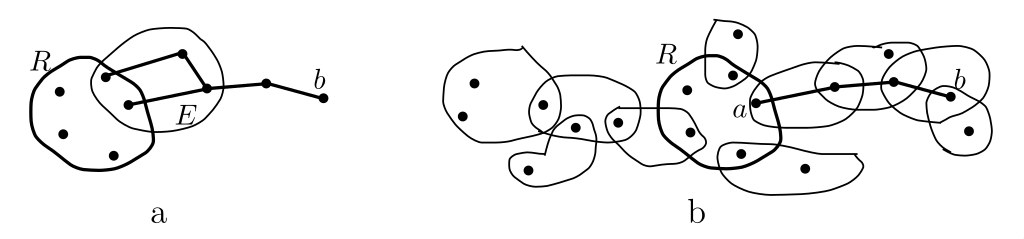
\includegraphics[width=0.6\columnwidth]{figures/theorem_1_3.png}
	\caption{Рисунок к 6 пункту Теоремы \ref{theorem:1_3}.}
    \label{fig:theorem_1_3}
\end{figure}

	Рассмотрим $R$ ~-- гиперребро $H$, $b \in V(H) \setminus R$.

	Посмотрим на все пути в $H$ от $b$ до гиперребра $R$, внутренние вершины которых не входят в $R$ и отметим множество всех их концов в гиперребре $R$.

	Пусть мы отметили хотя бы две вершины из  $R$, тогда в $H$ существует цикл $Z$ содержащий ровно две отмеченные вершины и хотя бы одну вершину не из $R$, смотреть Рис. \ref{fig:theorem_1_3} (а).

	Следовательно, существует и гиперребро $E$, содержащее все вершины $Z$.
	Это гиперребро не совпадает с  $R$ и  $|E \cap R| \geqslant 2 \implies $ противоречие пункту 2.

	Значит, каждый путь в  $H$ от $b$ до гиперребра $R$, внутренние вершины которого не входят в $R$ имеет концом одну и ту же вершину $a \in R$, а значит  $a$ отделяет $b$ от  $r$.
 \end{proof}

\subsection{Гипердерево разбиения. Теорема о разбиении.}

\begin{df*}
	Рассмотрим конечное множество вершин $V$. Пусть каждой вершине $w \in V$ соответствует разбиение $V_w$ множества $V \setminus \{w\}$ на несколько \textbf{классов}(возможно на один).

	Будем говорить, что вершина $w$ \textbf{разделяет} вершины $v_1$ и $v_2$, если $v_1$ и $v_2$ лежат в разных классах $V_w$.

	И называть  $V$ \textbf{множеством с разбиением}.
\end{df*}

\begin{df*}[Гиперграф разбиения, $\Struct(V)$]
	Назовем вершины $v_1,v_2 \in V$ \textbf{соседними}, если их не разделяет никакая отличная от них вершина из $V$.

	Построим \textbf{гиперграф разбиения}  $\Struct(V)$  на вершинах множества $V$, гиперребра которого это максимальные по включению множества попарно соседних вершин.
\end{df*}

\begin{df*}[Индуцированное разбиение]
	Для любого $W \subset V$ определим \textbf{индуцированное разбиение}: для каждой вершины $x \in W$ положим $W_x = V_x \cap W$.
\end{df*}

\begin{customthm}{1.4} \label{theorem:1_4}
	Если для любых $a, b, c \in V$ таких, что  $a$ разделяет $b$ и $c$, верно что  $b$ не разделяет $a$ и $c$.

	Тогда выполнены следующие утверждения:

	\begin{enumerate}
		\item Гиперграф $\Struct(V)$ является гипердеревом
		\item Пусть для некоторой вершины $a \in V$ гиперграф $\Struct(V) - a$ распадается на компоненты связности $W_1, \ldots, W_l$, тогда $V_a = \{W_1, \ldots, W_l\}$
	\end{enumerate}
\end{customthm}

В условиях Теоремы \ref{theorem:1_4} докажем вспомогательные утверждения.

\begin{customclaim}{1.1} \label{claim:1_1}
	Существуют вершины $a, b \in V \colon |V_a| = |V_b| = 1$
\end{customclaim}

\begin{proof}
	Индукция по количеству вершин в $V$. База для множества состоящего из двух вершин очевидна. 

	Рассмотрим теперь произвольную вершину $c \in V$, пусть  $V' = V \setminus\{c\}$.

	Для каждой вершины $x \in V'$ положим $V_x' = V_x \setminus \{c\}$.

	По индукционному предположению существуют вершины $a, b \in V' \colon |V_a'| = |V_b'| = 1$, если  $|V_a| = |V_b| = 1$, то утверждение доказано, предположим обратное.

	Пусть  $|V_a| > 1$, тогда вершина  $a$ разделяет $V' \setminus \{a\} \ni b$ и  $c$, а значит по условию получаем что $b$ не разделяет $a$ и $c$ а значит $|V_b| = 1$.

	Для любой вершины  $x \in V' \setminus \{a\}$ вершина $a$ разделяет $c$ и $x$, следовательно, вершина  $c$ не разделяет $a$ и $x$, таким образом $|V_c| = 1$ и вершины $b, c$ нам подходят. 
\end{proof}

\begin{customclaim}{1.2} \label{claim:1_2}
	Гиперграф $\Struct(V)$ связен.
\end{customclaim}

\begin{proof}
	Базой считаем множество состоящее не более чем из трех вершин.

	Рассмотрим вершины $a, b \in V \colon |V_a| = |V_b| = 1$, по Утверждению \ref{claim:1_1}.

	По индукции гиперграф  $\Struct(V \setminus \{a\})$ связен, т.к. $|V_a| = 1$, то все вершины множества  $V \setminus \{a\}$ связаны, и в гиперграфе $\Struct(V)$.
	По аналогичным причинам, вершины множества $V \setminus \{b\}$ связаны в $\Struct(V)$, а значит связен и весь $\Struct(V)$.
\end{proof}

\begin{customclaim}{1.3} \label{claim:1_3}
	Пусть $a_1a_2 \ldots a_k$ ~-- путь в гиперграфе $\Struct(V)$, а вершины $b$ не лежит на нем. Тогда $b$ не разделяет $\{a_1, \ldots, a_k\}$.
\end{customclaim}

\begin{proof}
	Заметим, что $b$ не разделяет две вершины которые лежат в одном гиперребре, тогда вершина $b$ не разделяет пары соседних вершин $a_1$ и $a_2$, $a_2$ и $a_3$, $\ldots$,  $a_{k - 1}$ и  $a_k$.
\end{proof}

\begin{proof}[\normalfont\textsc{Доказательство Теоремы \ref{theorem:1_4}}]
	По Утверждению \ref{claim:1_2} гиперграф $\Struct(V)$ связен.

	По Утверждению \ref{claim:1_3} любые две вершины, входящие в какой-либо цикл графа $\Struct(V)$, невозможно разделить никакой отличной от них вершиной.

	Следовательно, все вершины цикла принадлежат одному гиперребру, в силу максимальности гиперребер(т.е. того что они максимальны по включению).

	А значит $\Struct(V)$ является гипердеревом и тогда первый пункт верен.

	Рассмотрим теперь множество $W_i$ - компонента связности графа  $\Struct(V) - a$.
	По Утверждению \ref{claim:1_3}  $a$ не разделяет никакие две вершины из $W_i$, а значит все вершины из $W_i$ лежат в одном классе разбиения $V_a$.

	Рассмотрим две разные компоненты  $W_i, W_j$ и выберем в них смежные с  $a$ вершины $w_i, w_j$ соответственно. Смотреть Рис. \ref{fig:theorem_1_4}.

\begin{figure}[ht]
    \centering
	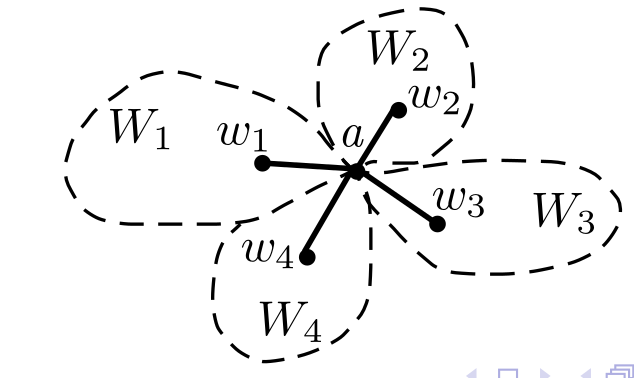
\includegraphics[width=0.4\columnwidth]{figures/theorem_1_4.png}
	\caption{Рисунок ко второму пункту Теоремы \ref{theorem:1_4}.}
    \label{fig:theorem_1_4}
\end{figure}

никакая отличная от $w_i, w_j, a$ вершина не может разделить пары смежных вершин  $\{w_i, a\}$ и  $\{w_j, a\}$. Следовательно, разделить вершины  $w_i, w_j$ может только  $a$.

Поскольку  $w_i$ и  $w_j$ не принадлежат одному гиперребру(ведь в разных компонентах связности графа $\Struct(V) - a$), то $a$ их разделяет, следовательно, все вершины $W_i$ лежат в одной компоненте связности, а  $W_j$ в другой.


\end{proof}

\end{document}
